\selectlanguage{italian}

La Fisica Statistica (quantistica) fornisce le relazioni tra le proprietà medie microscopiche di un sistema con le sua dinamica macroscopica. In particolare, si fanno due assunzioni fondamentali (per rendere la trattazione indipendente dalle condizioni iniziali del sistema):
\begin{enumerate}
	\item equilibrio: il sistema ha superato tutti i transienti e tutte le quantità collettive (es.: pressione) hanno delle piccole fluttuazioni attorno ad un valore ben definito;
	\item ergodicità: le medie temporali delle osservabili coincidono con le medie d'ensemble.
\end{enumerate}

\section{Operatore densità}

Si consideri un sistema quantistico di $ N $ corpi (con $ N \sim N_\text{A} \simeq 6.022 \cdot 10^{23} $). Detti $ \{\ket{\psi_i}\}_{i \in \mathcal{I}} $ i possibili stati in cui si può trovare il sistema e detta $ w_i \in [0,1] $ la probabilità che il sistema si trovi in $ \ket{\psi_i} $ (condizione di normalizzazione $ \sum_{i \in \mathcal{I}} w_i = 1 $), l'\textit{expectation value} di un'osservabile $ \hat{B} $ sarà:
\begin{equation}
	[B] \defeq \sum_{i \in \mathcal{I}} w_i \braket{\psi_i | \hat{B} | \psi_i}
\end{equation}
Data un set completo ortonormale $ \{\ket{b_j}\}_{j \in \mathcal{J}} $ di autostati di $ \hat{B} $, allora $ \hat{B} = \sum_{j \in \mathcal{J}} b_j \ket{b_j}\bra{b_j} $, ovvero:
\begin{equation}
	[B] = \sum_{i \in \mathcal{I}} \sum_{j \in \mathcal{J}} w_i b_j \abs{\braket{b_j | \psi_i}}^2
	\label{eq:b-exp-val}
\end{equation}

\begin{definition}{Operatore densità}{}
	Si definisce l'\textit{operatore statistico} (o operatore densità) come:
	\begin{equation}
		\hat{\rho} \defeq \sum_{i \in \mathcal{I}} w_i \ket{\psi_i}\bra{\psi_i}
	\end{equation}
\end{definition}

\begin{theorem}{Expectation value}{}
	L'expectation value di un'osservabile $ \hat{B} $ può essere espresso come:
	\begin{equation}
		[B] = \tr(\hat{\rho} \hat{B})
	\end{equation}

	\tcblower

	\begin{proof}
		Dall'Eq. \ref{eq:b-exp-val} (e ricordando che $ \{\ket{b_j}\}_{j \in \mathcal{J}} $ è base ortonormale di $ \hilb $):
		\begin{equation*}
			[B] = \sum_{i \in \mathcal{I}} \sum_{j \in \mathcal{J}} w_i b_j \braket{b_j | \psi_i} \braket{\psi_i | b_j} = \sum_{j \in \mathcal{J}} b_j \braket{b_j | \hat{\rho} | b_j} = \sum_{j \in \mathcal{J}} \braket{b_j | \hat{\rho} \hat{B} | b_j} \eqdef \tr(\hat{\rho} \hat{B})
		\end{equation*}
	\end{proof}
\end{theorem}

Un corollario banale è che $ \tr{\hat{\rho}} = 1 $ (con $ \hat{B} \equiv \id_\hilb $). Inoltre, si vede che per un sistema in uno stato puro, ovvero $ w_i = \delta_{i,i_0} $ per un certo $ i_0 \in \mathcal{I} $, allora $ \hat{\rho} = \ket{\psi_{i_0}}\bra{\psi_{i_0}} $ è un proiettore (dunque idempotente: $ \hat{\rho}^2 = \hat{\rho} $).

\section{Ensemble all'equilibrio}

\subsection{Ensemble microcanonico}

Si consideri un sistema isolato ad energia fissata $ E $ con una piccola incertezza $ \Delta E $: questo viene detto \textit{ensemble microcanonico}. Dall'ipotesi di ergodicità deriva che tutti gli stati amessi dalla conservazione dell'energia sono equiprobabili:
\begin{equation}
	w_i =
	\begin{cases}
		\frac{1}{\Omega} & E_i \in [E - \Delta E/2 , E + \Delta E/2] \\
		0 & E_i \notin [E - \Delta E/2 , E + \Delta E/2]
	\end{cases}
	\label{eq:microcanon-ens}
\end{equation}
dove $ \Omega = \Omega(E, \Delta E) $ è il numero di stati accessibili nello spazio delle fasi posta la condizione energetica.

\subsection{Ensemble canonico}

Si consideri ora un sistema $ \text{S} $ al'interno dell'universo $ \text{U} $ e sia $ \text{W} \equiv \text{U} - \text{S} $. Assumendo che $ \mathcal{H}_\text{U} = \mathcal{H}_\text{S} + \mathcal{H}_\text{W} + \mathcal{H}_\text{SW} \approx \mathcal{H}_\text{S} + \mathcal{H}_\text{W} $, ovvero che sia $ \text{S} $ che $ \text{U} $ siano considerabili isolati, allora questi saranno descritti dalla distribuzione microcanonica Eq. \ref{eq:microcanon-ens}.

\begin{theorem}{Distribuzione canonica}{}
	Dato uno stato possibile $ \ket{\psi_m} $ con energia $ E_m $ del sistema $ \text{S} $, la sua probabilità è data dalla \textit{distribuzione di Boltzmann}:
	\begin{equation}
		P_m^\text{S} = \frac{1}{Z} e^{- \beta E_m}
	\end{equation}
	dove $ \beta = \beta(T) $ e $ Z $ è la \textit{funzione di partizione} del sistema $ \text{S} $:
	\begin{equation}
		Z \defeq \sum_{i \in \mathcal{I}} e^{- \beta E_i} \equiv \tr e^{- \beta \mathcal{H}}
		\label{eq:part-func-states}
	\end{equation}

	\tcblower

	\begin{proof}
		Dall'ipotesi di interazione debole tra $ \text{S} $ e $ \text{W} $ si ha $ P^\text{U}(E) = P^\text{S}(E_m) P^\text{W}(E - E_m) $, dunque, essendo questi sistemi microcanonici:
		\begin{equation*}
			P_m^\text{S} = \frac{P^\text{U}(E)}{P^\text{W}(E-E_m)} = \frac{\Omega_\text{W}(E-E_m,\Delta E)}{\Omega_\text{U}(E,\Delta E)}
		\end{equation*}
		Assumendo $ E_m \ll E $ si può sviluppare in serie:
		\begin{equation*}
			\ln \Omega_\text{W}(E - E_m , \Delta E) = \ln \Omega_\text{W}(E , \Delta E) - \beta E_m + o(E_m^2)
			\qquad \qquad
			\beta \equiv \frac{\pa}{\pa x}\bigg\vert_{x = E} \ln \Omega_\text{W}(x , \Delta E)
		\end{equation*}
		Esponenziando e sostituendo nell'equazione precedente si ottiene:
		\begin{equation*}
			P_m^\text{S} = \frac{\Omega_\text{W}(E , \Delta E)}{\Omega_\text{U}(E, \Delta E)} e^{- \beta E_m} \equiv \frac{1}{Z} e^{- \beta E_m}
		\end{equation*}
		Il fattore iniziale non dipende da $ \ket{m} $, dunque è un fattore puramente di normalizzazione. Dalla condizione di normalizzazione $ \sum_{i \in \mathcal{I}} P_i^\text{S} = 1 $ si trova la tesi.
	\end{proof}
\end{theorem}

Si noti che nell'Eq. \ref{eq:part-func-states} la sommatoria è su tutti gli stati, includendo in particolare quelli degeneri. Si può passare ad una sommatoria sulle energie ammesse definendo la degenerazione del livello energetico $ E $ come $ g(E) $, così che:
\begin{equation}
	Z = \sum_E g(E) e^{- \beta E}
\end{equation}
Inoltre, sebbene $ P_m^\text{S} $ dipenda da tutti i possibili valori di energia, il rapporto di probabilità $ P_m^\text{S} / P_n^\text{S} = e^{-\beta (E_m - E_n)} $ dipende solo da $ \Delta E_{mn} \equiv E_m - E_n $. \\
L'operatore densità dell'ensemble canonico (di Gibbs) è diagonale nell'autobase di $ \mathcal{H} $:
\begin{equation}
	\hat{\rho}_\text{Gibbs} = \sum_{m \in \mathcal{I}} \frac{e^{-\beta E_m}}{Z} \ket{m}\bra{m} \equiv \frac{e^{-\beta \mathcal{H}}}{\tr e^{-\beta \mathcal{H}}}
	\label{eq:op-dens-gibbs}
\end{equation}

\begin{example}{Sottosistemi isolati}{}
	Si consideri $ \text{S} = \text{S}_1 \cup \text{S}_2 $, con $ \text{S}_1 $ ed $ \text{S}_2 $ isolati. Allora:
	\begin{equation*}
		P_{(m_1,m_2)}^\text{S} = P_{m_1}^{\text{S}_1} P_{m_2}^{\text{S}_2} = \frac{1}{Z_1 Z_2} e^{-\beta (E_{m_1} + E_{m_2})}
	\end{equation*}
	confermando che $ E_{(m_1,m_2)} = E_{m_1} + E_{m_2} $ ($ \beta_1 = \beta_2 = \beta $ all'equilibrio). Dunque la distribuzione di Boltzmann riproduce i risultati intuitivi. Si noti inoltre che la funzione di partizione è una funzione moltiplicativa ($ Z_{1,2} = Z_1 Z_2 $), così che il suo logaritmo sia additivo ($ \ln Z_{1,2} = \ln Z_1 + \ln Z_2 $).
\end{example}

\subsection{Termodinamica}

È possibile ricavare le principali quantità termodinamiche a partire dalla funzione di partizione e dall'operatore densità.

\begin{proposition}{Energia interna}{}
	L'energia interna media è:
	\begin{equation}
		U = - \frac{\pa}{\pa \beta} \ln Z
	\end{equation}

	\tcblower

	\begin{proof}
		Definendo $ U \equiv [\mathcal{H}] $:
		\begin{equation*}
			U = \tr(\hat{\rho}_\text{Gibbs} \mathcal{H}) = \sum_{m \in \mathcal{I}} P_m E_m = \frac{\sum_{m \in \mathcal{I}} E_m e^{-\beta E_m}}{\sum_{m \in \mathcal{I}} e^{- \beta E_m}} = - \frac{1}{Z} \frac{\pa Z}{\pa \beta} = - \frac{\pa}{\pa \beta} \ln Z
		\end{equation*}
	\end{proof}
\end{proposition}

Essendo $ \ln Z $ additivo su sistemi isolati, l'energia interna è correttamente una quantità termodinamica estensiva. Si vede inoltre che l'energia interna è una funzione non crescente di $ \beta $:
\begin{equation*}
	\frac{\pa U}{\pa \beta} = - \frac{\pa^2}{\pa \beta^2} Z = \frac{1}{Z^2} \left[ -Z \sum_{m \in \mathcal{I}} E_m^2 e^{-\beta E_m} + \left( \sum_{m \in \mathcal{I}} E_m e^{-\beta E_m} \right)^2 \right] = - [\mathcal{H}^2] + [\mathcal{H}]^2 = - [(\mathcal{H} - [\mathcal{H}])^2] \le 0
\end{equation*}

\begin{lemma}[before upper = {\tcbtitle}]{}{}
	\begin{equation}
		\beta = \frac{1}{k_\text{B} T}
	\end{equation}

	\tcblower

	\begin{proof}
		Si definisca l'energia libera $ F \equiv - \frac{1}{\beta} \ln Z $, così che $ U = \frac{\pa}{\pa \beta} (\beta F) $. D'altro canto, dalla Termodinamica si ha $ U - TS = F $, con $ S = - \frac{\pa F}{\pa T} $ l'entropia, dunque:
		\begin{equation*}
			\frac{F}{T} = \frac{U}{T} - S
			\quad \Rightarrow \quad
			U = \frac{\pa}{\pa(1/T)} \frac{F}{T} = \frac{\pa}{\pa \beta} (\beta F)
			\quad \Rightarrow \quad
			\beta \propto \frac{1}{T}
		\end{equation*}
		Nel limite classico si trova la corretta costante di proporzionalità.
	\end{proof}
\end{lemma}

\begin{proposition}{Calore specifico}{}
	Il calore specifico (a volume costante) è:
	\begin{equation}
		c_V = k_\text{B} \beta^2 \frac{\pa^2}{\pa \beta^2} \ln Z
	\end{equation}

	\tcblower

	\begin{proof}
		Ricordando che $ c_V \defeq \frac{\pa U}{\pa T} $ basta notare che $ \frac{\pa}{\pa T} = \frac{\pa \beta}{\pa T} \frac{\pa}{\pa \beta} = - \frac{1}{k_\text{B} T^2} \frac{\pa}{\pa \beta^2} $, ovvero:
		\begin{equation}
			\frac{\pa}{\pa T} = - k_\text{B} \beta^2 \frac{\pa}{\pa \beta}
		\end{equation}
	\end{proof}
\end{proposition}

È anche possibile dare una definizione più generale di entropia. Innanzitutto, dato che $ F = U - TS $, per l'ensemble canonico si trova:
\begin{equation}
	S = \frac{U}{T} - k_\text{B} \ln Z
	\label{eq:entropy-canon-ens}
\end{equation}
Questa può però essere generalizzata anche per sistemi non all'equilibrio.

\begin{definition}{Entropia}{}
	Dato un sistema con operatore densità $ \hat{\rho} $, si definisce l'\textit{entropia} come:
	\begin{equation}
		S \defeq - k_\text{B} \tr(\hat{\rho} \ln \hat{\rho})
	\end{equation}
\end{definition}

Sulla base degli autostati di $ \hat{\rho} $ (autostati $ \ket{\rho_m} $ con autovalori $ P_m $), l'entropia è:
\begin{equation}
	S = - k_\text{B} \sum_{m \in \mathcal{I}} P_m \ln P_m
\end{equation}

\begin{example}{Stato puro}{}
	Per uno stato puro $ P_m = \delta_{m,m_0} $, dunque correttamente $ S = -k_\text{B} \ln 1 = 0 $.
\end{example}

\begin{example}{Ensemble microcanonico}{}
	Per un ensemble microcanonico $ P_m = \frac{1}{\Omega} \,\,\forall m \in \mathcal{I} \,:\, \abs{\mathcal{I}} = \Omega $, dunque:
	\begin{equation*}
		S = - k_\text{B} \sum_{m = 1}^\Omega \frac{1}{\Omega} \ln \frac{1}{\Omega} = k_\text{B} \Omega \frac{1}{\Omega} \ln \Omega = k_\text{B} \ln \Omega
	\end{equation*}
	che è proprio l'equazione di Boltzmann.
\end{example}

\begin{example}{Ensemble canonico}{}
	Per l'ensemble canonico l'operatore densità è quello di Gibbs (Eq. \ref{eq:op-dens-gibbs}):
	\begin{equation*}
		S = - k_\text{B} \sum_{m \in \mathcal{I}} \frac{e^{-\beta E_m}}{Z} \ln \frac{e^{-\beta E_m}}{Z} = \frac{k_\text{B}}{Z} \sum_{m \in \mathcal{I}} e^{-\beta E_m} (\beta E_m + \ln Z) = k_\text{B} \beta [\mathcal{H}] + k_\text{B} \frac{Z \ln Z}{Z} = \frac{U}{T} + k_\text{B} \ln Z
	\end{equation*}
	che coincide con l'Eq. \ref{eq:entropy-canon-ens}. Si può dimostrare che $ \hat{\rho}_\text{Gibbs} $ è l'operatore densità che massimizza l'entropia per una data $ U = \tr(\hat{\rho}\mathcal{H}) $ fissata (oltre a $ N $ e $ V $): questo conferma il secondo principio della termodinamica, poiché un sistema generico descritto da $ \hat{\rho} $ tenderà all'ensemble canonico, ovverosia all'equilibrio, massimizzando l'entropia.
\end{example}

\section{Sistemi ideali}

Un sistema di $ N $ particelle si dice \textit{ideale} se si può separare:
\begin{equation}
	\mathcal{H} = \sum_{i = 1}^N \mathcal{H}_i \,:\, [\mathcal{H}_i , \mathcal{H}_j] = 0
\end{equation}
dove $ \mathcal{H}_i $ descrive soltanto i gradi di libertà della particella $ i $-esima. Lo spettro di questa Hamiltoniana è $ E_{\alpha_1, \dots, \alpha_N} = E_{\alpha_1} + \dots + E_{\alpha_N} $, ed inoltre si definisce il numero di occupazione $ n_k $ del livello energetico $ E_k $, $ I \in \mathcal{N} \subset \N $, così da poter scrivere la funzione di partizione del sistema come:
\begin{equation}
	Z = \sum_{\alpha_1, \dots, \alpha_N \in \mathcal{I}} \frac{\prod_{k \in \mathcal{I}} n_k!}{N!} \exp \left( - \beta \sum_{i = 1}^N E_{\alpha_i} \right)
\end{equation}
Per un sistema bosonico la sommatoria su $ \alpha_1, \dots, \alpha_N $ non ha condizioni, mentre per un sistema fermionico essa è solo su $ \alpha_1 \neq \dots \neq \alpha_N $ (ed in tal caso $ n_k \in \{0,1\} \,\,\forall k \in \mathcal{I} $, ovvero $ n_k! = 1 \,\,\forall k \in \mathcal{I} $). Questa funzione di partizione non è fattorizzabile in generale, a causa della produttoria per i bosoni e del principio di Pauli per i fermioni, ma diventa fattorizzabile in particolari regimi. \\
Si assuma che lo spettro enegetico del sistema non abbia limite superiore: a bassa temperatura, il fattore esponenziale nella distribuzione di Boltzmann tende a favorire stati con energia totale $ \sum_{i = 1}^N E_{\alpha_i} = \sum_{\alpha \in \mathcal{I}} n_\alpha E_\alpha $ più bassa; d'altro canto, ad alta temperatura, tutti gli stati single-particle con $ E_\alpha \lesssim k_\text{B} T $ hanno una probabilità pressoché eguale di essere occupati, e per $ T $ molto grande il numero di tali possibili stati è $ \gg N $, dunque la praticamente totalità degli stati a $ N $ particelle avranno soltanto stati con $ n_\alpha \in \{0,1\} $, indipendentemente dalla natura fermionica o bosonica del sistema. Ciò è riportato in Fig. \ref{boson-temp}. \\
Il limite classico (a $ Z $ separabile) può anche essere ottenuto agendo sulla densità del sistema: a parità di $ N $, sistemi con $ V $ maggiore avranno un maggior numero si stati accessibili: i gas ideali\footnote{I sistemi ideali possono essere solo in fase gassosa, poiché si ignora l'interazione tra particelle.} diventano classici o scaldandoli molto o rarefacendoli molto. Inoltre, a parità di densità e temperatura, un gas di particelle di massa inferiore avrà livelli energetici più vicini, dunque sarà più facilmente classico.

\begin{figure}
	\centering
	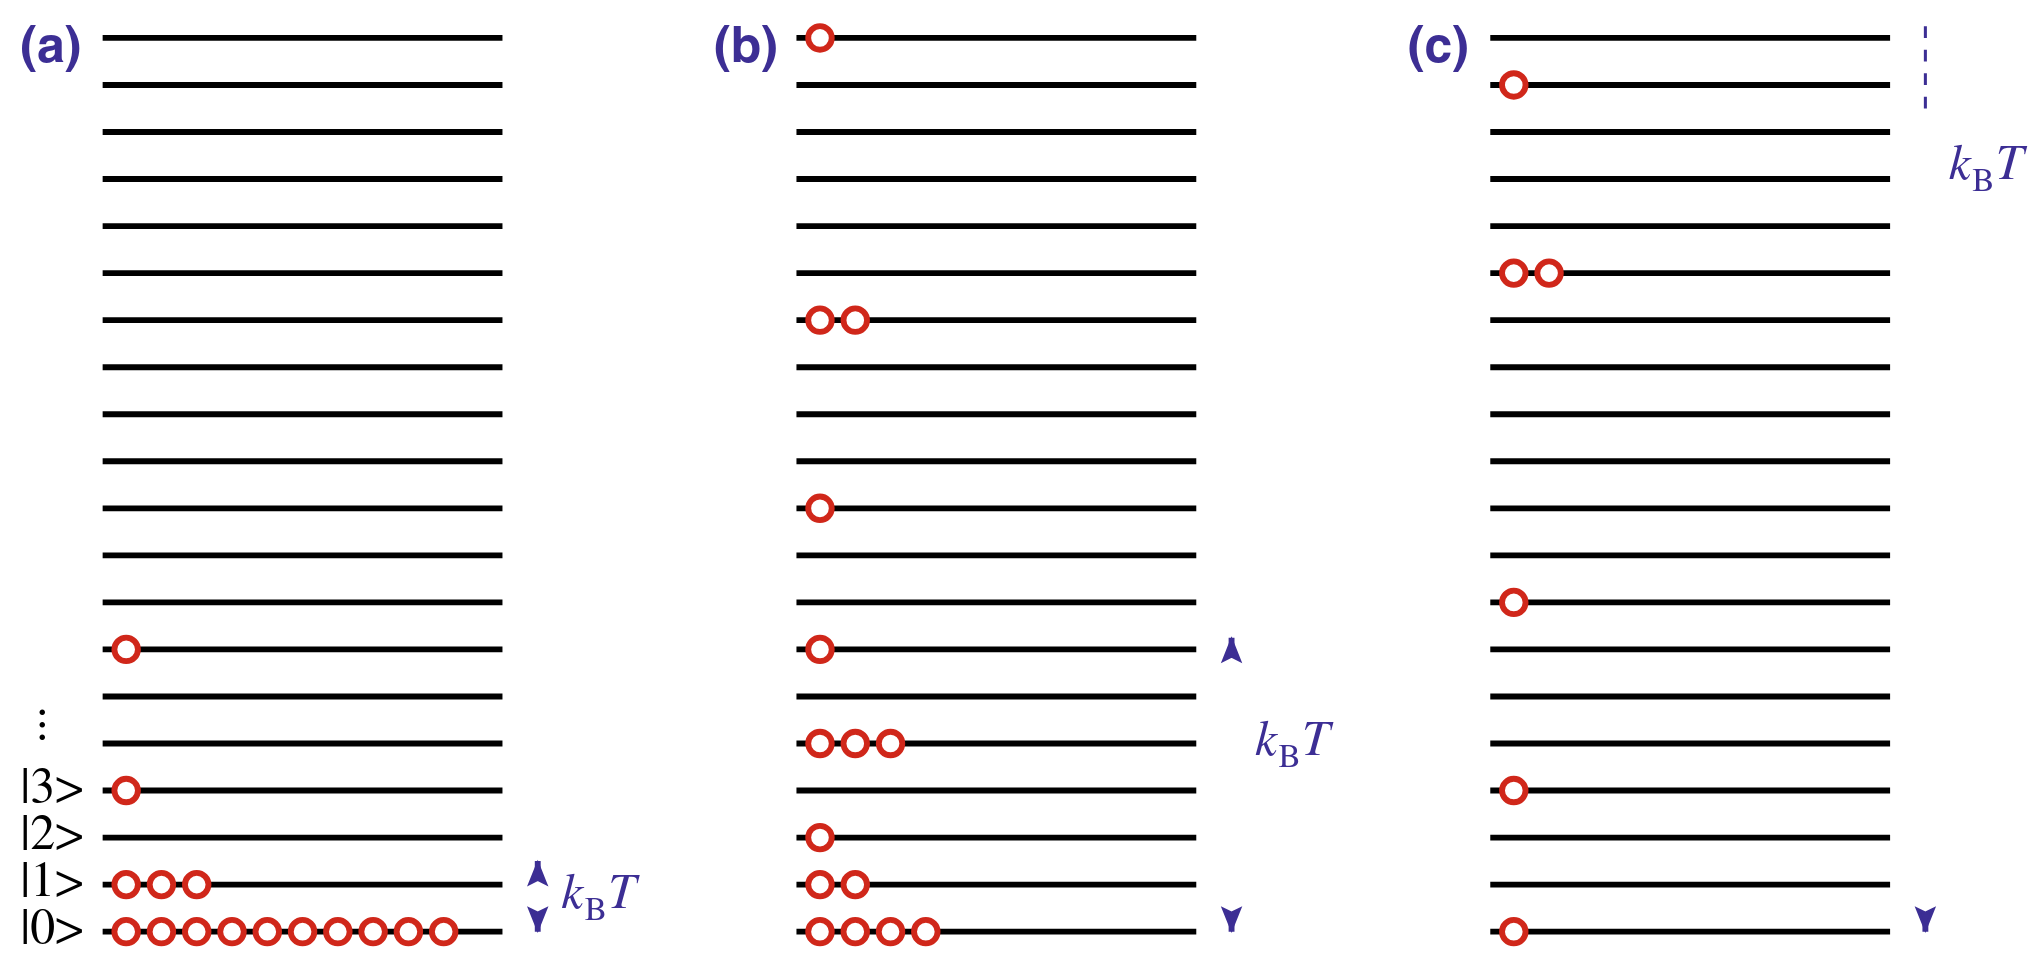
\includegraphics[width = 0.70 \textwidth]{ideal-high-temp.png}
	\caption{Occupancies of single-particle energy eigenstates for a bosonic system in the low-, intermediate- and high-temperature limits.}
	\label{boson-temp}
\end{figure}

\subsection{Limite ad alta temperatura}

Nel limite ad alta temperatura si può non tenere conto dell'occupazione degli stati, poiché il gas si comporta classicamente e $ n_\alpha \in \{0,1\} \,\,\forall \alpha \in \mathcal{I} $. Si ottiene dunque una funzione di partizione ad alta temperatura valida sia per fermioni che per bosoni:
\begin{equation}
	Z \simeq \frac{1}{N!} \sum_{\alpha_1, \dots, \alpha_N \in \mathcal{I}} \exp \left( -\beta \sum_{i = 1}^N E_{\alpha_i} \right) = \frac{1}{N!} \prod_{i = 1}^N Z_i \equiv \frac{Z_1^N}{N!}
\end{equation}
dove $ Z_1 $ è la funzione di partizione single-particle $ Z_1 \equiv \sum_{\alpha \in \mathcal{I}} \exp \left( -\beta E_\alpha \right) $. \\
Essendo in fase gassosa, il centro di massa di ciascuna particella si muove liberamente ed è dunque separabile dai gradi di libertà interni, ovvero $ \mathcal{H}_i = \mathcal{H}_{i,\text{tr}} + \mathcal{H}_{i,\text{int}} $ e $ Z_1 = Z_{1,\text{tr}} Z_{1,\text{int}} $: mentre $ Z_{1,\text{int}} $ dipende dallo specifico spettro di eccitazioni dei gradi di libertà interni, $ Z_{1,\text{tr}} $ è universale e dipende solo dalla massa della particella $ M $ e dal volume in cui si trova il sistema $ V $.

\subsubsection{Gradi di libertà traslazionali}

Si consideri una particella confinata in un cubo macroscopico di volume $ V = L^3 $ e si impongano delle condizioni al contorno periodiche, ovvero che la funzione d'onda è uguale su facce opposte del cubo. Le autofunzioni $ \psi_\ve{k}(\ve{r}) = L^{-3/2} \exp(i \ve{k} \cdot \ve{r}) $ possono avere solo valori quantizzati di $ \ve{k} $:
\begin{equation*}
	k_j = \frac{2\pi}{L} n_j \,\,,\,\, n_j \in \Z
\end{equation*}
L'energia cinetica traslazionale associata è:
\begin{equation}
	E_\ve{n} = \frac{\hbar^2 \ve{k}^2}{2M} = \frac{(2\pi\hbar)^2}{2M L^2} (n_x^2 + n_y^2 + n_z^2)
\end{equation}
Per $ L $ o $ M $ macroscopicamente grande (limite termodinamico) questo spettro diventa continuo:
\begin{equation*}
	\begin{split}
		Z_{1,\text{tr}}
		& = \sum_{\ve{n} \in \Z^3} e^{-\beta E_\ve{n}} = \sum_{\ve{n} \in \Z^3} \exp \left[ - \beta \frac{(2\pi\hbar)^2}{2M L^2} (n_x^2 + n_y^2 + n_z^2) \right] \\
		& \rightarrow \int_{\R^3} \dd n_x \dd n_y \dd n_z \exp \left[ -\beta \frac{(2\pi\hbar)^2}{2M L^2} (n_x^2 + n_y^2 + n_z^2) \right] = \left( \frac{L}{\hbar} \sqrt{\frac{M k_\text{B} T}{2\pi}} \right)^3
	\end{split}
\end{equation*}
Si può definire la \textit{lunghezza termica}:
\begin{equation}
	\Lambda \defeq \sqrt{\frac{2\pi\hbar^2}{M k_\text{B} T}}
\end{equation}
così da ottenere:
\begin{equation}
	Z_{1,\text{tr}} = \frac{V}{\Lambda^3}
\end{equation}
Si ha dunque:
\begin{equation*}
	Z = \frac{Z_1^N}{N!} = \frac{Z_{1,\text{tr}}^N}{N!} Z_{1,\text{int}}^N \equiv Z_\text{tr} Z_{1,\text{int}}^N
\end{equation*}

\begin{proposition}[before upper = {\tcbtitle}]{Energia interna traslazionale}{}
	\begin{equation}
		U_\text{tr} = \frac{3}{2} N k_\text{B} T
	\end{equation}

	\tcblower

	\begin{proof}
		\begin{equation*}
			\begin{split}
				U_\text{tr}
				& = - \frac{\pa}{\pa \beta} \ln Z_\text{tr} = - \frac{\pa}{\pa \beta} \ln \frac{V^N}{N! \Lambda^{3N}} = 3N \frac{\pa}{\pa \beta} \ln \Lambda = 3N \frac{\pa}{\pa \beta} \ln \sqrt{\beta} = \frac{3N}{2\beta} = \frac{3}{2} N k_\text{B} T
			\end{split}
		\end{equation*}
	\end{proof}
\end{proposition}

Ciò è in accordo con l'equipartizione dell'energia di Boltzmann.

\begin{theorem}{Equazione di stato dei gas perfetti}{}
	Per un gas perfetto vale l'equazione di stato:
	\begin{equation}
		P = \frac{N k_\text{B} T}{V}
	\end{equation}

	\tcblower

	\begin{proof}
		Innanzitutto, si trova l'energia libera nel limite ad alta temperatura:
		\begin{equation*}
			F \defeq - \frac{\ln Z}{\beta} \simeq - \frac{1}{\beta} \ln \frac{(Z_1)^N}{N!} = - \frac{1}{\beta} (N \ln Z_1 - \ln N!) \simeq - \frac{1}{\beta} (N \ln Z_1 - N \ln (N/e))
		\end{equation*}
		dove si è usata l'approssimazione di Stirling $ \ln N! \simeq N \ln (N/e) $. Dunque:
		\begin{equation}
			F = - N k_\text{B} T \ln \frac{e Z_1}{N}
		\end{equation}
		Per la pressione:
		\begin{equation*}
			\begin{split}
				P \defeq - \frac{\pa F}{\pa V} \bigg\vert_{T,N}
				& = - \frac{\pa}{\pa V} \bigg\vert_{T,N} \left[ - N k_\text{B} T \ln \frac{e Z_{1,\text{tr}} Z_{1,\text{int}}}{N} \right] = N k_\text{B} T \frac{\pa}{\pa V} \bigg\vert_{T,N} \left[ \ln \frac{eV}{N \Lambda^3} + \ln Z_{1,\text{int}} \right] \\
				& = N k_\text{B} T \frac{\pa}{\pa V}\bigg\vert_{T,N} \ln \frac{eV}{N \Lambda^3} = N k_\text{B} T \frac{1}{V}
			\end{split}
		\end{equation*}
	\end{proof}
\end{theorem}

Confrontando con $ pV = nRT $, essendo $ N = n N_\text{A} $, si trova $ k_\text{B} = R / N_\text{A} $.

\paragraph{Distribuzione energetica}

Per ricavare la distribuzione di Boltzmann delle energie cinetiche è necessario passare da un'integrale sugli stati $ \ve{n} $ ad un'integrale sull'energia $ E $. La densità degli stati nello spazio degli stati è:
\begin{equation}
	g(\ve{k}) = \frac{\dd n_x}{\dd k_x} \frac{\dd n_y}{\dd k_y} \frac{\dd n_z}{\dd k_z} = \frac{L^3}{8\pi^3} \equiv \frac{V}{8\pi^3}
\end{equation}
Si vede che gli stati sono distribuiti uniformemente. È necessario trovare la densità degli stati nello spazio delle energie tale per cui:
\begin{equation*}
	g(E) \dd E = g(\ve{k}) \dd^3\ve{k} = g(\ve{k}) 4\pi k^2 \dd k
\end{equation*}
Il differenziale $ \dd k $ si ottiene invertendo la relazione di dispersione $ E = E(k) $, che in questo caso dà:
\begin{equation*}
	k = \sqrt{\frac{2M E}{\hbar^2}}
	\quad \Rightarrow \quad
	\dd k = \sqrt{\frac{M}{2\hbar^2 E}} \dd E
\end{equation*}
Si ottiene dunque:
\begin{equation*}
	g(E) \dd E = \frac{V}{8\pi^3} 4 \pi \frac{2M E}{\hbar^2} \sqrt{\frac{M}{2\hbar^2 E}} \dd E = \frac{V M^{3/2}}{\sqrt{2} \pi^2 \hbar^3} \sqrt{E} \dd E
\end{equation*}
ovvero:
\begin{equation}
	g_\text{tr}(E) = \frac{V M^{3/2}}{\sqrt{2} \pi^2 \hbar^3} \sqrt{E}
\end{equation}
La distribuzione di probabilità che descrive l'energia di una singola particella si può trovare come:
\begin{equation*}
	\frac{\dd P(E)}{\dd E} = g_\text{tr}(E) \frac{e^{- \beta E}}{Z_{1,\text{tr}}} = \frac{V M^{3/2}}{\sqrt{2} \pi^2 \hbar^3} \sqrt{E} \frac{\Lambda^3}{V} e^{-\beta E}
\end{equation*}
Il risultato è indipendente dal volume e dalla massa della particella, ed è dunque universale (a parità di temperatura):
\begin{equation}
	\frac{\dd P(E)}{\dd E} = \frac{2}{\sqrt{\pi}} \beta^{3/2} \sqrt{E} e^{-\beta E}
	\label{eq:maxw-boltz-en}
\end{equation}
Si può ricavare anche una distribuzione delle velocità, trovando che ciascuna componente di $ \ve{v} = \frac{\ve{p}}{M} $ è distribuita gaussianamente come:
\begin{equation*}
	\frac{\dd P(v_j)}{\dd v_j} = \sqrt{\frac{\beta M}{2\pi}} \exp \left( -\beta \frac{M v_j^2}{2} \right)
\end{equation*}
La distribuzione di $ v \equiv \abs{\ve{v}} $ si trova dall'Eq. \ref{eq:maxw-boltz-en}:
\begin{equation*}
	\frac{\dd P(v)}{\dd v} = \frac{\dd P(E)}{\dd E} \frac{\dd E}{\dd v} = M v \frac{\dd P(E)}{\dd E}
\end{equation*}
Sostituendo $ E = \frac{1}{2} M v^2 $ si trova la \textit{distribuzione di Maxwell-Boltzmann}:
\begin{equation}
	\frac{\dd P(v)}{\dd v} = \sqrt{\frac{2 M^3}{\pi (k_\text{B} T)^3}} v^2 \exp \left( - \frac{M}{2 k_\text{B} T} v^2 \right)
\end{equation}










